%%%%%%%%%%%%%%%%%%%%%%%%%%%%%%%%%%%%%%%%%%%%%%%%%%%%%%%%%%%%%%%%%%%%%%%%%%%%%%%%
%2345678901234567890123456789012345678901234567890123456789012345678901234567890
%        1         2         3         4         5         6         7         8
%% PP_Report.tex
%% V2.1
%% 2017/05/07
%% by Rui Santos Cruz
%% This is a skeleton file using PPIEEEtran.cls
%% (requires PPIEEEtran.cls) 
% !TEX root = ./main.tex
%%%%%%%%%%%%%%%%%%%%%%%%%%%%%%%%%%%%%%%%%%%%%%%%%%%%%%%%%%%%%%%%%%%%%%%%%%%%%%%%
\documentclass[a4paper,12pt,journal,twoside,compsoc]{PPIEEEtran}

% In the ReportType command chose "act" for Activity Report or "learn" for Learnings Report
\newcommand*{\ReportType}{}
% -----------------------------------------------------------------------------
% The Preamble document contains all the necessary Packages for typesetting
% Modify it to suit your needs
% -----------------------------------------------------------------------------
%%%%%%%%%%%%%%%%%%%%%%%%%%%%%%%%%%%%%%%%%%%%%%%%%%%%%%%%%%%%%%%%%%%%%%%%%%%%%%%%
%2345678901234567890123456789012345678901234567890123456789012345678901234567890
%        1         2         3         4         5         6         7         8
% Required Packages and commands
% --> Please Choose the MAIN LANGUAGE for the document in package BABEL (below)
% --> Please Choose the TYPE OF REPORT for the document in \ReportType (below)
% !TEX root = ./main.tex
% PP_Report_Preamble.tex
% V2.1
% 2017/05/07
% by Rui Santos Cruz
%%%%%%%%%%%%%%%%%%%%%%%%%%%%%%%%%%%%%%%%%%%%%%%%%%%%%%%%%%%%%%%%%%%%%%%%%%%%%%%%
%
% *** INPUT LANGUAGE PACKAGES ***
% Choose the main language in package Babel
\usepackage[main=english,portuguese]{babel}
\usepackage[utf8]{inputenc}
\usepackage{iflang}

% *** ACRONYM PACKAGES ***
% Put definition of Acronyms at the end of the document
\usepackage[printonlyused,nolist]{acronym}

% *** CITATION PACKAGES ***
\usepackage{cite}

% *** GRAPHICS RELATED PACKAGES ***
\usepackage[pdftex]{graphicx}
\DeclareGraphicsExtensions{.pdf,.jpeg,.png}

% *** MATH PACKAGES ***
\usepackage[cmex10]{amsmath}

% *** SPECIALIZED LIST PACKAGES ***
\usepackage{algorithmic}

% *** ALIGNMENT PACKAGES ***
\usepackage{array}

% *** SUBFIGURE PACKAGES ***
\usepackage[caption=false,font=normalsize,labelfont=sf,textfont=sf]{subfig}

% *** FLOAT PACKAGES ***
\usepackage{fixltx2e}

% *** PDF, URL AND HYPERLINK PACKAGES ***
\usepackage{url}

% *** BACKGROUND Material ***
\usepackage{eso-pic}
\usepackage[
  contents={},
  opacity=1,
  scale=1,
  color=blue!90
  ]{background}
  
% *** CONDITIONALS ***
\usepackage{ifthen}

% Clever Referencing
% Note: portuguese is supported through "brazilian" option
\usepackage[\IfLanguageName{english}{english}{brazilian}]{cleveref}

%%%%%%%%%%%%%%%%%%%%%%%%%%%%%%%%%%%%%%%%%%%%%%%%%%%%%%%%%%%%%%%%%%%%%%%%%%%%%%%%
% PLEASE DO NOT CHANGE THIS SECTION
% Printing the Scoring Table
\AddToShipoutPicture*{\BackgroundPic}
%%%%%%%%%%%%%%%%%%%%%%%%%%%%%%%%%%%%%%%%%%%%%%%%%%%%%%%%%%%%%%%%%%%%%%%%%%%%%%%%
% PLEASE DO NOT CHANGE THIS SECTION
% Print Vertical Identifications on even and odd pages
\AddEverypageHook{%
  \ifthenelse{\isodd{\value{page}}}%
  {\backgroundsetup{
    angle=90,
    position={-0.1\textwidth,-1.055\textheight},
    contents={\tiny{PP-2017 V2.1}}
    }% Odd Pages
  }%
  {\backgroundsetup{
    angle=90,
    position={0.97\textwidth,-1.05\textheight},%
    contents={\ifthenelse{\equal{\ReportType}{act}}{%
              \tiny{\tlangRepActivity}}{\tiny{\tlangRepLearning}}}
    }% Even Pages
  }%
  \BgMaterial}
  %%%%%%%%%%%%%%%%%%%%%%%%%%%%%%%%%%%%%%%%%%%%%%%%%%%%%%%%%%%%%%%%%%%%%%%%%%%%%%%%
% correct bad hyphenation here
\hyphenation{op-tical net-works semi-conduc-tor}
%%%%%%%%%%%%%%%%%%%%%%%%%%%%%%%%%%%%%%%%%%%%%%%%%%%%%%%%%%%%%%%%%%%%%%%%%%%%%%%%
%2345678901234567890123456789012345678901234567890123456789012345678901234567890
%        1         2         3         4         5         6         7         8
\begin{document}

%%%%%%%%%%%%%%%%%%%%%%%%%%%%%%%%%%%%%%%%%%%%%%%%%%%%%%%%%%%%%%%%%%%%%%%%%%%%%%%%
%2345678901234567890123456789012345678901234567890123456789012345678901234567890
%        1         2         3         4         5         6         7         8
%% PP_Report_Cover.tex
%% V2.1
%% 2017/05/07
%% by Rui Santos Cruz
% !TEX root = ./main.tex
%%%%%%%%%%%%%%%%%%%%%%%%%%%%%%%%%%%%%%%%%%%%%%%%%%%%%%%%%%%%%%%%%%%%%%%%%%%%%%%%
% paper title
% can use linebreaks \\ within to get better formatting as desired
% Do not put math or special symbols in the title.
\title{Cloud Security: Asigurarea securit\u{a}\c{t}ii multi-tenant \^{i}n servicii cloud}

%%%%%%%%%%%%%%%%%%%%%%%%%%%%%%%%%%%%%%%%%%%%%%%%%%%%%%%%%%%%%%%%%%%%%%%%%%%%%%%%
% Author names
%
% note positions of commas and nonbreaking spaces ( ~ ) LaTeX will not break
% a structure at a ~ so this keeps an author's name from being broken across
% two lines.
% use \thanks{} to gain access to the first footnote area
% a separate \thanks must be used for each paragraph.
%
%\IEEEcompsocitemizethanks is a special \thanks that produces the bulleted
% lists for "first footnote" author affiliations. 
% Use \IEEEcompsocthanksitem which works much like \item
% for each affiliation group.
\author{Pricop~Gabriela~Florina,
        
% Change the Course Name 
% note: need leading \protect in front of \\ to get a newline within \thanks as
% \\ is fragile and will error, could use \hfil\break instead.
\IEEEcompsocitemizethanks{
\IEEEcompsocthanksitem Pricop~Gabriela~Florina\protect\\ 
E-mail: gabriela.florina.pr@gmail.com,

Inginerie Software, Universitatea Tehnica Cluj-Napoca.\protect\\}% <-this % stops an unwanted space}% <-this % stops an unwanted space
\thanks{Manuscript received on Month Day, 2999.}
}
%%%%%%%%%%%%%%%%%%%%%%%%%%%%%%%%%%%%%%%%%%%%%%%%%%%%%%%%%%%%%%%%%%%%%%%%%%%%%%%%
% The paper headers
\markboth{Multi-tenancy security}%
% for a single student
%{Surname}% : for a single student 
% for a Group Report 
{Gabriela}% : for a Group Report 
%
% The only time the second header will appear is for the odd numbered pages
% after the title page when using the twoside option.

%%%%%%%%%%%%%%%%%%%%%%%%%%%%%%%%%%%%%%%%%%%%%%%%%%%%%%%%%%%%%%%%%%%%%%%%%%%%%%%%
% Prints in Subtitle the type of Report
% PLEASE DO NOT CHANGE THIS SECTION
\IEEEspecialpapernotice{%
\ifthenelse{\equal{\ReportType}{act}}{%
\tlangRepActivity}{\tlangRepLearning}
}
%%%%%%%%%%%%%%%%%%%%%%%%%%%%%%%%%%%%%%%%%%%%%%%%%%%%%%%%%%%%%%%%%%%%%%%%%%%%%%%%
%%%%%%%%%%%%%%%%%%%%%%%%%%%%%%%%%%%%%%%%%%%%%%%%%%%%%%%%%%%%%%%%%%%%%%%%%%%%%%%%
% The paper Abstract and Keywords
\IEEEtitleabstractindextext{%

\begin{abstract}
The Abstract should not exceed 200 words and should not be an introductory text on the subject of the report, but a summary of the whole report, describing what the author(s) did, how it was done, the main results and their importance. It should be discursive and not just a list of topics covered in the report.
\end{abstract}
%
\begin{IEEEkeywords}
 
\end{IEEEkeywords}}
%%%%%%%%%%%%%%%%%%%%%%%%%%%%%%%%%%%%%%%%%%%%%%%%%%%%%%%%%%%%%%%%%%%%%%%%%%%%%%%%

% make the title area
\maketitle

\IEEEdisplaynontitleabstractindextext
\IEEEpeerreviewmaketitle
%%%%%%%%%%%%%%%%%%%%%%%%%%%%%%%%%%%%%%%%%%%%%%%%%%%%%%%%%%%%%%%%%%%%%%%%%%%%%%%%
%%%%%%%%%%%%%%%%%%%%%%%%%%%%%%%%%%%%%%%%%%%%%%%%%%%%%%%%%%%%%%%%%%%%%%%%%%%%%%%%
\section{Introduction}
% The very first letter is a 2 line initial drop letter followed
% by the rest of the first word in caps (small caps for compsoc).
% 
% form to use if the first word consists of a single letter:
% \IEEEPARstart{A}{demo} file is ....
% 
% Here we have the typical use of a "E" for an initial drop letter
% and "STE" in caps to complete the first word.
\IEEEPARstart{T}{his} demo file is intended to serve as a ``starter file''
for writing the Activity\slash Learning Reports of Independent Studies, produced under \LaTeX\ using
IEEEtrans class template.

The objective of what you have done with your activity is thought of as ``providing experience, provoking reflection''.

The extra-curricular activity that you have performed provided an experience where you learned about the entity or community partner as well as about the work. But you also learned about yourself and reflection is about deriving meaning and knowledge from the experience. But reflection can be a challenging endeavor, as it is not something that is fostered in classes, where someone (the teacher) tells you (the student) how you are doing! At best, students can typically narrate what they did, but have trouble thinking abstractly about their learning–-patterns, connections and progress.

\begin{figure}[htb]
\centering
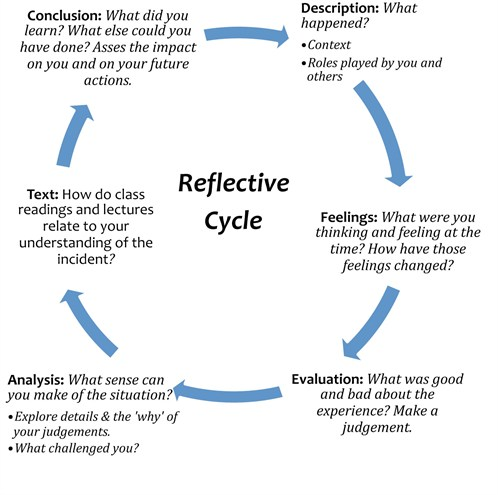
\includegraphics[width=1\linewidth]{reflective-cycle.jpg}
\caption{The Reflectice Cycle}
\label{fig_ref_cycle}
\end{figure}

It is therefore the objective of these Reports to enhance your experiential learnings, through a factual ``description'' of what you have done (basically the Activity Report), and an ``evaluation'' and ``analysis'' of what you have experienced (basically, the Learnings Report), see \Cref{fig_ref_cycle}.\\

This document is organized as follows. \Cref{rubrics} describes the scoring Rubrics. \Cref{features} illustrates some features you can use. \Cref{dummy} is just a dummy text for illustration purposes, and \Cref{concl} concludes the report.

%%%%%%%%%%%%%%%%%%%%%%%%%%%%%%%%%%%%%%%%%%%%%%%%%%%%%%%%%%%%%%%%%%%%%%%%%%%%%%%%
\section{Scoring Rubrics}
\label{rubrics}
The table of Scoring Rubrics (at the bottom of the first page of each Report) depends on the Report Type (ACTIVITY or LEARNINGS). Therefore, you must pay attention to have the correct table displayed when you select your Report Type in line 15 of the \textbf{PP\_Report.tex} document. Failure to do so means that your Report WILL NOT BE ACCEPTED for evaluation.

The scoring Rubrics correspond to the evaluation of different aspects of your Reports, and have the following meanings.

In the Activity Report:
\begin{description}
\item[ACTIVITY table]  \hfill \\
This table contains the rubrics that evaluate the Activity Report as an objective, factual document, describing the purpose of the activity, the tasks performed, the execution environment, the constraints, results etc. 
\begin{itemize}
\item[\textbf{Intro}] This rubric evaluates how you introduce the Activity described in the document. A competent introduction should describe at least the significance of the topic and the purposes of the work. 
\item[\textbf{Object}] This rubric evaluates how you describe what were the Objectives of the work, and how you planned/prepared it. 
\item[\textbf{Tasks}] This rubric evaluates if you provide clear and concise description of the procedures/tasks that were performed.
\item[\textbf{Exec}] This rubrics will evaluate how you describe all the phases/steps of the work/activity, and will consider items such as when, where, how, what, with/for whom, duration, etc.
\item[\textbf{Result}] This rubric will evaluate how you describe the results of the work performed. You should report your results neutrally.
\end{itemize}
\end{description}

In the Learnings Report:
\begin{description}
\item[LEARNINGS table] \hfill \\
This table contains the rubrics that evaluate your learning experience in terms of non-technical (soft) skills acquired or perfected.
\begin{itemize}
\item[\textbf{Intro}] This rubric evaluates how you introduce the subject (your own experience) to be described. A competent introduction should describe at least the significance of what you have done and what you have learned from doing it.
\item[\textbf{Motiv}] This rubric evaluates how you describe your motivation for choosing and performing the activity.
\item[\textbf{Skills}] This rubric evaluates how you describe all the soft-skills, perfected and/or acquired, during the execution of the activity.
\item[\textbf{Reflect}] This rubric corresponds to the way you evaluate your experience, what was good and bad about it, and how well you describe it.
\item[\textbf{Analy}] This rubric evaluate your Analysis of the situation, on what sense can you make of it, what challenged you, and the ``why'' of your judgements (expressed in the Reflection part).
\end{itemize}
\end{description}


In both Reports:
\begin{description}
\item[DOCUMENT table] \hfill \\
This table contains the rubrics that evaluate the document form and structure.
\begin{itemize}
\item[\textbf{Struct}] Evaluation the structure of the document in terms of contents. Please note that wrongly formatted Appendixes (if existing) and Bibliography, as well as missing biographies (mini CV) and photos of the authors, are penalized.
\item[\textbf{Ortog}] Evaluates the quality of the orthography (spelling, appropriateness, etc.).
\item[\textbf{Gram}] Evaluates the grammar construction.
\item[\textbf{Form}] Evaluates the format conformance of the document in terms of components.
\item[\textbf{Abstr}] Evaluates the quality of the Abstract, if it is \textbf{really} a summary of the document. The abstract is what is initially previewed by readership to determine if the remainder of the document is worth reading. 
\item[\textbf{Concl}] This rubric evaluates how concise and analytic you are on drawing conclusions from what you have learned, what you have done or what else could you have done, assessing the impact on you and on your future actions. The Conclusion is comprised of some final, summative statements that reflect the flow and outcomes of the subject described in the document. 
\end{itemize}
\item[PENALTY table] \hfill \\
This table contains the rubrics related with the Titles of the document, file names and identification(s) of  author(s).
\begin{itemize}
\item[\textbf{Titles}] Evaluates if the Main Title, subtitle, abridged title, etc. are adequate.
\item[\textbf{Files}] Evaluates conformation of the file names of the submitted documents with the rules.
\item[\textbf{IDs}] Evaluates the correct information related with the identification of author(s), submission dates, etc.
\end{itemize}
\end{description}

%%%%%%%%%%%%%%%%%%%%%%%%%%%%%%%%%%%%%%%%%%%%%%%%%%%%%%%%%%%%%%%%%%%%%%%%%%%%%%%%
%%%%%%%%%%%%%%%%%%%%%%%%%%%%%%%%%%%%%%%%%%%%%%%%%%%%%%%%%%%%%%%%%%%%%%%%%%%%%%%%
\section{Features}
\label{features}
This section describes some of the common features used on writing documents with \LaTeX.
\subsection{Abbreviations and Acronyms} 
This template is ready to define abbreviations and acronyms the first time they are used in the text, even after they have been defined in the abstract.
For the students of \ac{IST} it becomes very easy to make references to the School just using the respective acronym. The first time it was used, in previous paragraph, the name of \ac{IST} was presented in extended form, but now only the acronym was typed.
%%%%%%%%%%%%%%%%%%%%%%%%%%%%%%%%%%%%%%%%%%%%%%%%%%%%%%%%%%%%%%%%%%%%%%%%%%%%%%%%
\subsection{Equations}
Writing equations or math expressions, for example $\alpha + \beta = \chi$, is also very easy.

Another method to write math expressions or equations is the following construct, normally numbered automatically:
\begin{equation}
\delta + \epsilon = \theta
\label{eq2}
\end{equation}

With this construct the reference in text to Equation~\ref{eq2} is straightforward.
%%%%%%%%%%%%%%%%%%%%%%%%%%%%%%%%%%%%%%%%%%%%%%%%%%%%%%%%%%%%%%%%%%%%%%%%%%%%%%%%
\subsection{Figures}
Placing figures is also very easy, as for example the following \Cref{fig_sim}:

\begin{figure}[htbp]
\centering
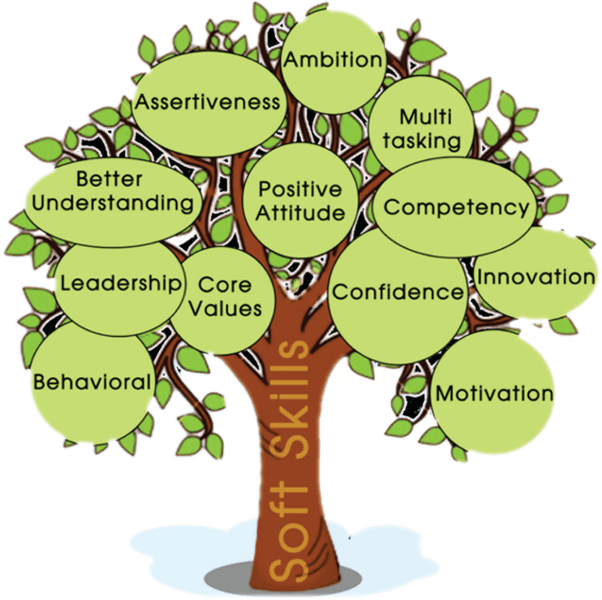
\includegraphics[width=1\linewidth]{soft_skills.png}
\caption{The Soft-Skills Tree}
\label{fig_sim}
\end{figure}

With this construct the reference in text to \Cref{fig_sim} is straightforward
%%%%%%%%%%%%%%%%%%%%%%%%%%%%%%%%%%%%%%%%%%%%%%%%%%%%%%%%%%%%%%%%%%%%%%%%%%%%%%%%
\section{Another Section}
\label{dummy}
Write here Some text. Note that some special characters need an escape sequence. For example, to write a \% sign you need to escape the character with a backslash (\textbackslash\%).
Cras sed sapien quam. Sed dapibus est id enim facilisis, at posuere turpis adipiscing. Quisque sit amet dui dui.
Duis rhoncus velit nec est condimentum feugiat. Donec aliquam augue nec gravida lobortis. Nunc arcu mi, pretium quis dolor id, iaculis euismod ligula. Donec tincidunt gravida lacus eget lacinia. 

Cras sed sapien quam. Sed dapibus est id enim facilisis, at posuere turpis adipiscing. Quisque sit amet dui dui.
Duis rhoncus velit nec est condimentum feugiat. Donec aliquam augue nec gravida lobortis. Nunc arcu mi, pretium quis dolor id, iaculis euismod ligula. Donec tincidunt gravida lacus eget lacinia. 
%%%%%%%%%%%%%%%%%%%%%%%%%%%%%%%%%%%%%%%%%%%%%%%%%%%%%%%%%%%%%%%%%%%%%%%%%%%%%%%%
\subsection{Now a Subsection}
Write here Some text. This is a bibliographic citation \cite{RFC_INTSERV}.
Duis rhoncus velit nec est condimentum feugiat. Donec aliquam augue nec gravida lobortis. Nunc arcu mi, pretium quis dolor id, iaculis euismod ligula. Donec tincidunt gravida lacus eget lacinia.

Cras sed sapien quam. Sed dapibus est id enim facilisis, at posuere turpis adipiscing. Quisque sit amet dui dui.
Duis rhoncus velit nec est condimentum feugiat. Donec aliquam augue nec gravida lobortis. Nunc arcu mi, pretium quis dolor id, iaculis euismod ligula. Donec tincidunt gravida lacus eget lacinia. 
\subsection{Yes Another Subsection}
Write here Some text. This is another bibliographic citation \cite{lamport:latex}. Donec aliquam augue nec gravida lobortis. Nunc arcu mi, pretium quis dolor id, iaculis euismod ligula. Donec tincidunt gravida lacus eget lacinia. 

Lorem ipsum dolor sit amet, consectetur adipiscing elit. Cras sed sapien quam. Sed dapibus est id enim facilisis, at posuere turpis adipiscing. Quisque sit amet dui dui \cite{lamport:latex}.

Duis rhoncus velit nec est condimentum feugiat. Donec aliquam augue nec gravida lobortis. Nunc arcu mi, pretium quis dolor id, iaculis euismod ligula. Donec tincidunt gravida lacus eget lacinia.
%%%%%%%%%%%%%%%%%%%%%%%%%%%%%%%%%%%%%%%%%%%%%%%%%%%%%%%%%%%%%%%%%%%%%%%%%%%%%%%%
\section{\IfLanguageName{english}{Conclusion}{Conclusão}}
\label{concl}
The conclusions. Lorem ipsum dolor sit amet, consectetur adipiscing elit. Cras sed sapien quam. Sed dapibus est id enim facilisis, at posuere turpis adipiscing. Quisque sit amet dui dui.

Duis rhoncus velit nec est condimentum feugiat. Donec aliquam augue nec gravida lobortis. Nunc arcu mi, pretium quis dolor id, iaculis euismod ligula. Donec tincidunt gravida lacus eget lacinia. Lorem ipsum dolor sit amet, consectetur adipiscing elit.


%%%%%%%%%%%%%%%%%%%%%%%%%%%%%%%%%%%%%%%%%%%%%%%%%%%%%%%%%%%%%%%%%%%%%%%%%%%%%%%%
% use section* for acknowledgement
\ifCLASSOPTIONcompsoc
  % The Computer Society usually uses the plural form
  \section*{\IfLanguageName{english}{Acknowledgments}{Agradecimentos}} % Acknowledgments
\else
  % regular IEEE prefers the singular form
  \section*{Acknowledgment}
\fi

The authors would like to thank...Lorem ipsum dolor sit amet, consectetur adipiscing elit. Cras sed sapien quam. Sed dapibus est id enim facilisis, at posuere turpis adipiscing. Quisque sit amet dui dui.
Duis rhoncus velit nec est condimentum feugiat. Donec aliquam augue nec gravida lobortis. Nunc arcu mi, pretium quis dolor id, iaculis euismod ligula. Donec tincidunt gravida lacus eget lacinia.
%%%%%%%%%%%%%%%%%%%%%%%%%%%%%%%%%%%%%%%%%%%%%%%%%%%%%%%%%%%%%%%%%%%%%%%%%%%%%%%%

% references section
\bibliographystyle{IEEEtran}
%\bibliography{PP_Report_bib}
\bibliography{Mendeley}
%%%%%%%%%%%%%%%%%%%%%%%%%%%%%%%%%%%%%%%%%%%%%%%%%%%%%%%%%%%%%%%%%%%%%%%%%%%%%%%%
% biography section
% 

\begin{IEEEbiography}[{
\includegraphics[width=1in,height=1.25in,clip,keepaspectratio]{me.png}}]{Name of Student One}
Here I am. I am pursuing my Engineering studies at \ac{IST}. Lorem ipsum dolor sit amet, consectetur adipiscing elit. Cras sed sapien quam. Sed dapibus est id enim facilisis, at posuere turpis adipiscing. Quisque sit amet dui dui. Lorem ipsum dolor sit amet, consectetur adipiscing elit. 
\end{IEEEbiography}


\begin{IEEEbiography}
[{
\includegraphics[width=1in,height=1.25in,clip,keepaspectratio]{me.png}}]{Name of Student Two}
Here I am. I am pursuing my Engineering studies at \ac{IST}. Lorem ipsum dolor sit amet, consectetur adipiscing elit. Cras sed sapien quam. Sed dapibus est id enim facilisis, at posuere turpis adipiscing. Quisque sit amet dui dui.Lorem ipsum dolor sit amet, consectetur adipiscing elit. 
\end{IEEEbiography}
%%%%%%%%%%%%%%%%%%%%%%%%%%%%%%%%%%%%%%%%%%%%%%%%%%%%%%%%%%%%%%%%%%%%%%%%%%%%%%%%
\newpage
\onecolumn
%%%%%%%%%%%%%%%%%%%%%%%%%%%%%%%%%%%%%%%%%%%%%%%%%%%%%%%%%%%%%%%%%%%%%%%%%%%%%%%%
% APPENDIX WITH STATEMENT OF EXECUTION IS ONLY
% MANDATORY FOR SELF_INITIATIVE ACTIVITIES
\appendix[Statements of Execution]
STATEMENT OF EXECUTION IS ONLY MANDATORY FOR SELF-INITIATIVE ACTIVITIES.

Place here your Statements of Execution of the Activity, using a PDF document.
\begin{figure*}[h]
\centering
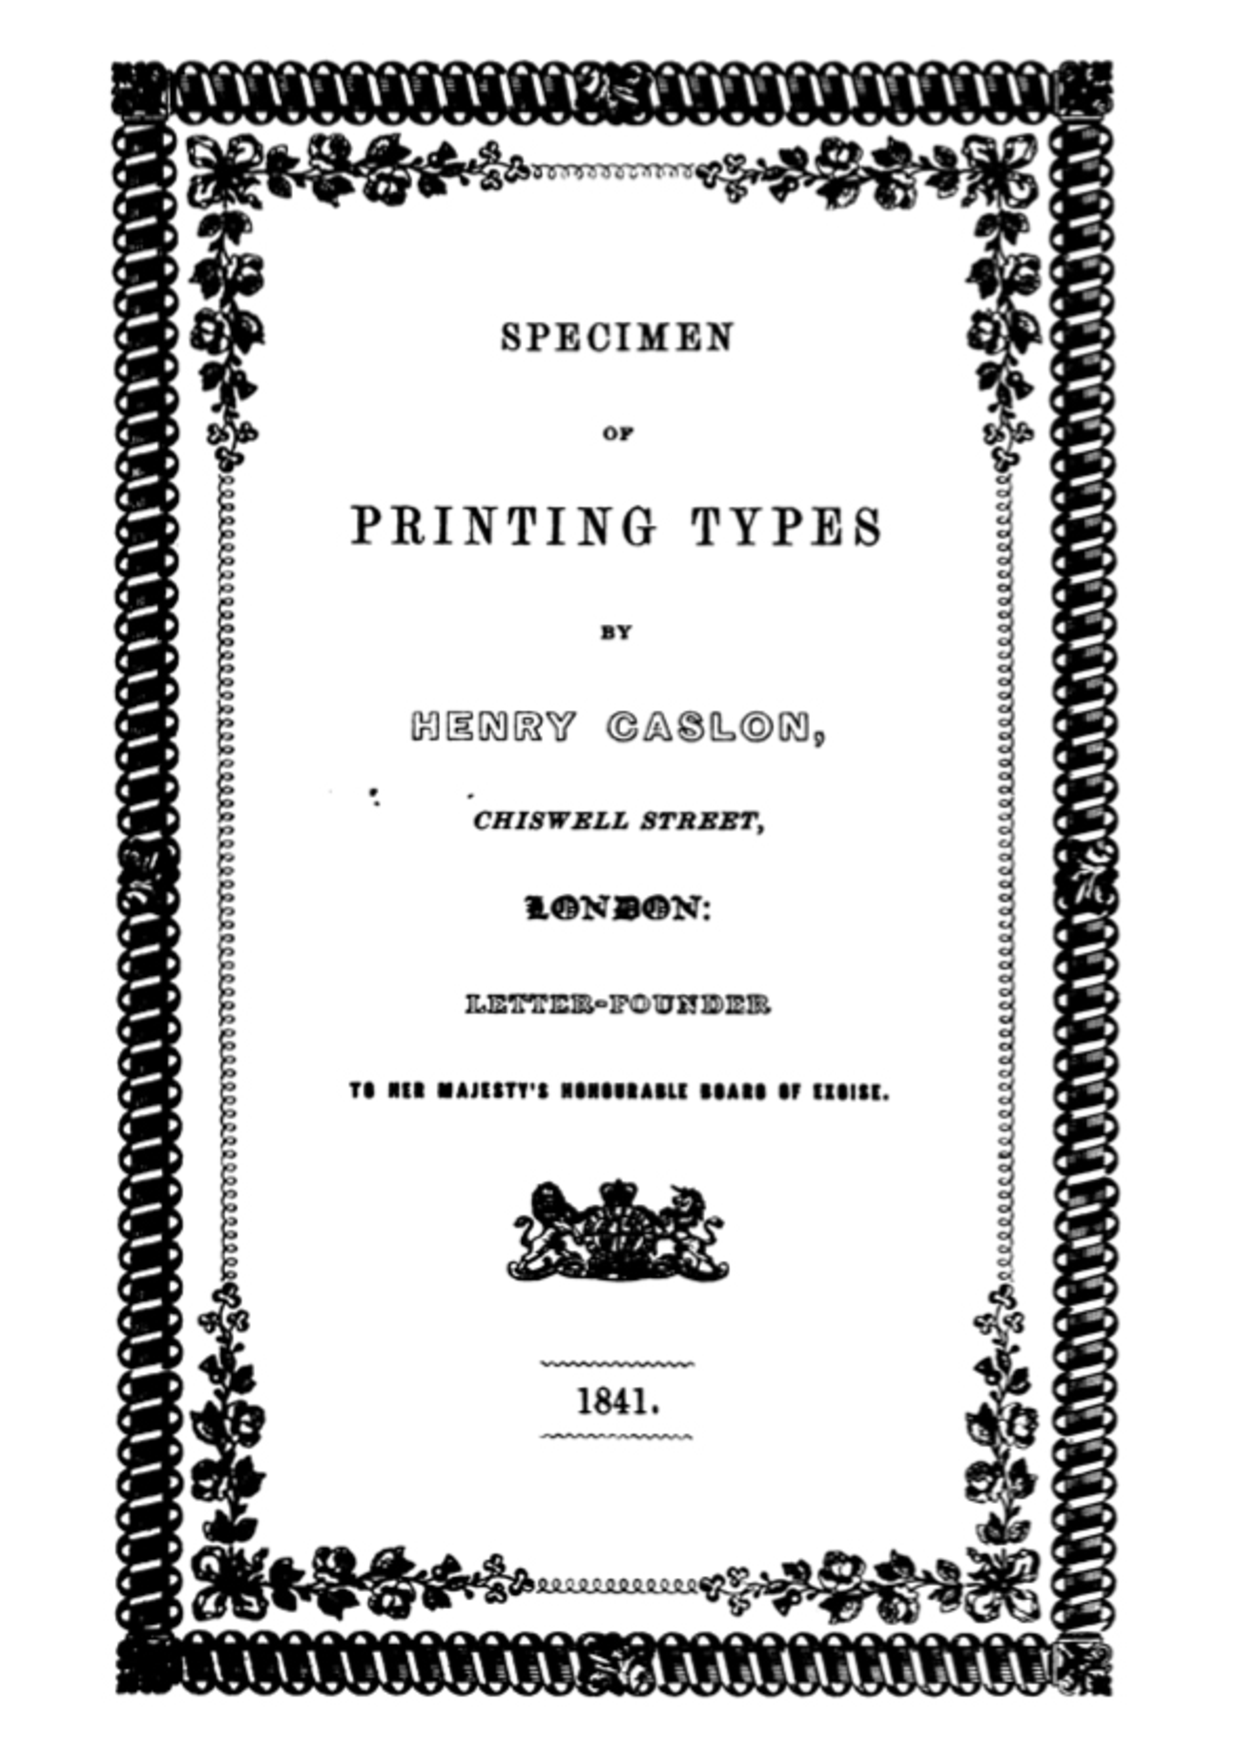
\includegraphics[width=0.8\textwidth]{specimen.pdf}
\end{figure*}
%%%%%%%%%%%%%%%%%%%%%%%%%%%%%%%%%%%%%%%%%%%%%%%%%%%%%%%%%%%%%%%%%%%%%%%%%%%%%%%%
% *** DEFINITION OF ACRONYMS ***
	\acrodef{CPU}{Central Processing Unit}
	\acrodef{GUI}{Graphical User Interface}
	\acrodef{HTTP}{Hypertext Transfer Protocol}
	\acrodef{IST}{Instituto Superior Técnico}	
	\acrodef{LAN}{Local Area Network}
	\acrodef{PC}{Personal Computer}
	\acrodef{URL}{Uniform Resource Locator}
	\acrodef{VoD}{Video-on-demand}
	\acrodefplural{VoD}[VoDs]{Videos-on-demand}
	\acrodef{VoIP}{Voice over IP}
	\acrodef{WAN}{Wide Area Network}
	\acrodef{WLAN}{Wireless Local Area Network}
	\acrodef{WWAN}{Wireless Wide Area Network}
	\acrodef{WWW}{World Wide Web}
	
% that's all folks
\end{document}